\section{Empirical Evaluation}
\label{section:evaluation}
Please showcase your empirical results in this section. Please clearly specify which sets of experiments of the original paper are considered in your report. Please also report the corresponding hyperparameters of each experiment.


1. remove the entropy term
2. remove \emph{trust region constraint}
In the environment of CartPole and MountainCarContinuous, the removal of trust region constraint from the algorithm seems to be better, especially in the MountainCarContinuous environment.
3. drop the bias term 
In both environment, the result with bias term dropped turns out to be significantly worse.
4. remove the clamping on the actor loss
5. change the \emph{truncation parameter}
6. change $Q_opc$ to $Q_ret$ 
7. change $Q_ret$ to $Q_opc$
8. change the power term of truncated importance weight from $1/d$ to $1 / e^d$
9. replace sdn structure to two independent networks

\begin{figure}
    \centering
    \subfigure[no clamp]{
        \centering
        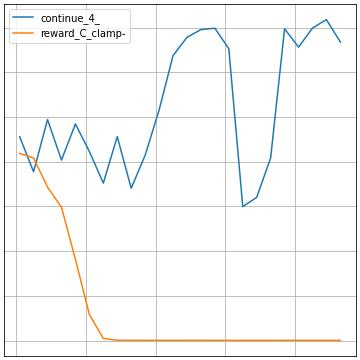
\includegraphics[width=0.225\textwidth]{continuous/clamp.jpg}        
    }            
    \hfill
    \subfigure[$d \rightarrow e^d$]{
        \centering
        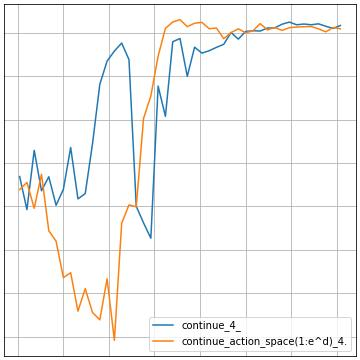
\includegraphics[width=0.225\textwidth]{continuous/e^d.jpg}
    }            
    \hfill
    \subfigure[no bias term]{
        \centering
        \includegraphics[width=0.225\textwidth]{continuous/no_bias_term.jpg}
    }  
    \hfill                
    \subfigure[no trust region]{
        \centering
        \includegraphics[width=0.225\textwidth]{continuous/no_trust_region.jpg}
    }                  
    \caption{continuous}    
    \label{fig:continous}
\end{figure}

\begin{figure}
    \centering
    \subfigure[$\text{truncation param} = 1$]{
        \centering
        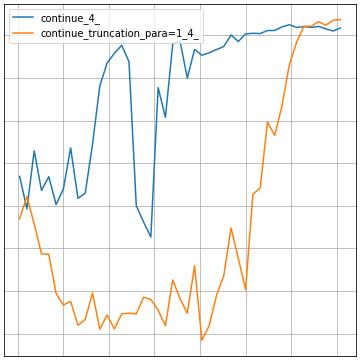
\includegraphics[width=0.3\textwidth]{continuous/continue_truncation_para=1.jpg}        
    }            
    \hfill
    \subfigure[$\text{truncation param} = 10$]{
        \centering
        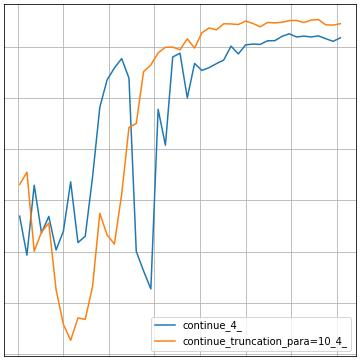
\includegraphics[width=0.3\textwidth]{continuous/continue_truncation_para=10.jpg}
    }            
    \hfill
    \subfigure[$\text{truncation param} = 15$]{
        \centering
        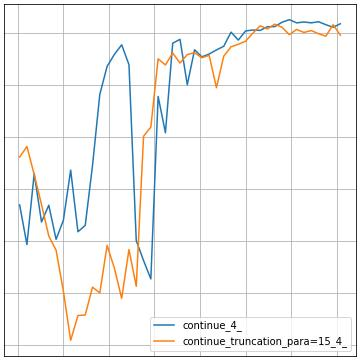
\includegraphics[width=0.3\textwidth]{continuous/continue_truncation_para=15.jpg}
    }  
    \caption{continous truncation param}    
    \label{fig:continous truncation param}
\end{figure}



\begin{figure}
    \centering
    \subfigure[$Q_{opc} \rightarrow Q_{ret}$]{
        \centering
        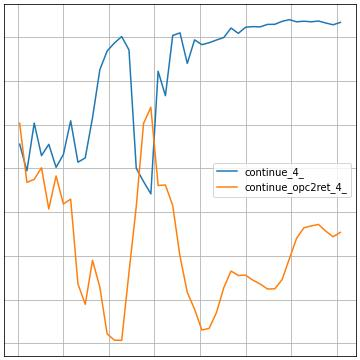
\includegraphics[width=0.45\textwidth]{continuous/opc2ret.jpg}        
    }            
    \hfill
    \subfigure[$Q_{ret} \rightarrow Q_{opc}$]{
        \centering
        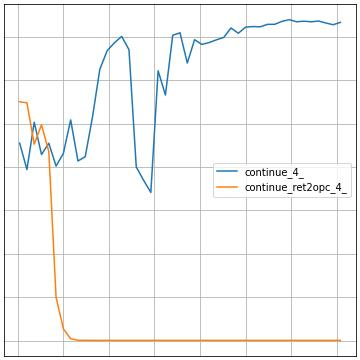
\includegraphics[width=0.45\textwidth]{continuous/ret2opc.jpg}
    }            
    \caption{opc and ret}    
    \label{fig: opc and ret}
\end{figure}


\begin{figure}
\caption{no sdn}
\centering
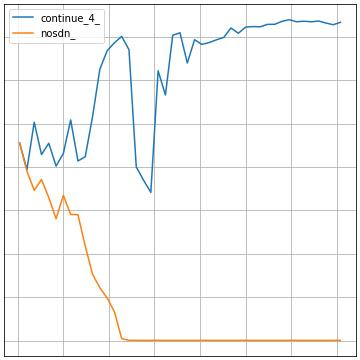
\includegraphics[width=0.5\textwidth]{continuous/nosdn.jpg}
\end{figure}



\begin{figure}
    \centering
    \subfigure[$\text{truncation param} = 1$]{
        \centering
        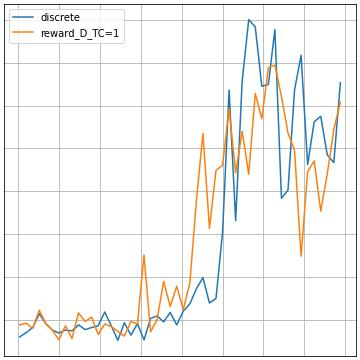
\includegraphics[width=0.3\textwidth]{discrete/D_TC=1.jpg}        
    }            
    \hfill
    \subfigure[$\text{truncation param} = 5$]{
        \centering
        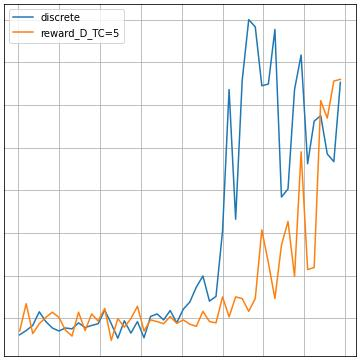
\includegraphics[width=0.3\textwidth]{discrete/D_TC=5.jpg}
    }            
    \hfill
    \subfigure[$\text{truncation param} = 20$]{
        \centering
        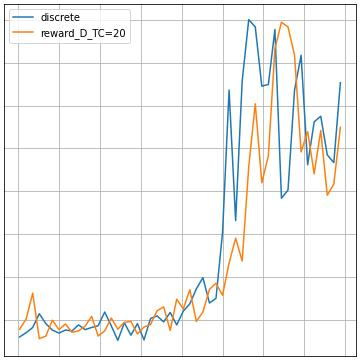
\includegraphics[width=0.3\textwidth]{discrete/D_TC=20.jpg}
    }  
    \caption{discrete truncation param, default = 10}    
    \label{fig:discrete truncation param}
\end{figure}


\begin{figure}
    \centering
    \subfigure[no clamp]{
        \centering
        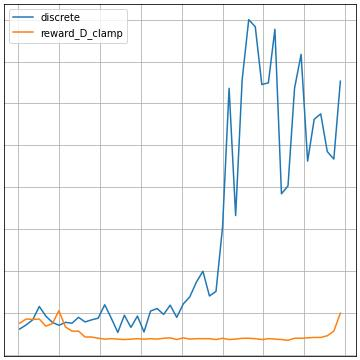
\includegraphics[width=0.3\textwidth]{discrete/D_clamp.jpg}
    }            
    \hfill
    \subfigure[no bias term]{
        \centering
        \includegraphics[width=0.3\textwidth]{discrete/no_bias_term.jpg}
    }            
    \hfill
    \subfigure[no trust region]{
        \centering
        \includegraphics[width=0.3\textwidth]{discrete/no_trust_region.jpg}
    }  
    \caption{discrete}    
    \label{fig:discrete}
\end{figure}


\begin{figure}
\caption{$Q_{ret} \rightarrow Q_{opc}$}
\centering
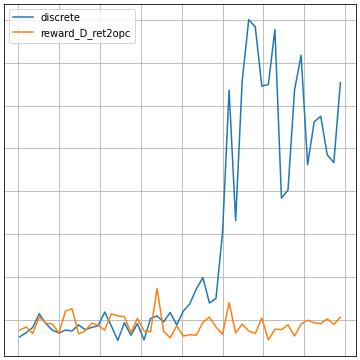
\includegraphics[width=0.5\textwidth]{discrete/D_ret2opc.jpg}
\end{figure}

    
As we can conclude, the algorithm is insensitive to the hyper-parameter tuning. 